\subsection{Définitions générales}
\framewithtitle{Définitions générales}

\begin{frame}{Contexte historique : origines de la blockchain}
  \begin{columns}
    \begin{column}{0.6\textwidth}
      \begin{itemize}
        \item 2008 : Satoshi Nakamoto publie \href{https://bitcoin.org/bitcoin.pdf}{\textquote{Bitcoin: A Peer-to-Peer Electronic Cash System}}
        \item Dans ces neuf pages, Nakamoto décris un système financier et introduit les bases de la blockchain
              \begin{itemize}
                \item Structure en blocs
                \item Cryptographie (hachage, asymmétrique, arbres de Merkel...)
                \item Transactions
              \end{itemize}
        \item Fun fact : Satoshi Nakamoto est toujours resté anonyme
      \end{itemize}
    \end{column}
    \begin{column}{0.4\textwidth}
      \begin{figure}
  \resizebox{\textwidth}{!}{
    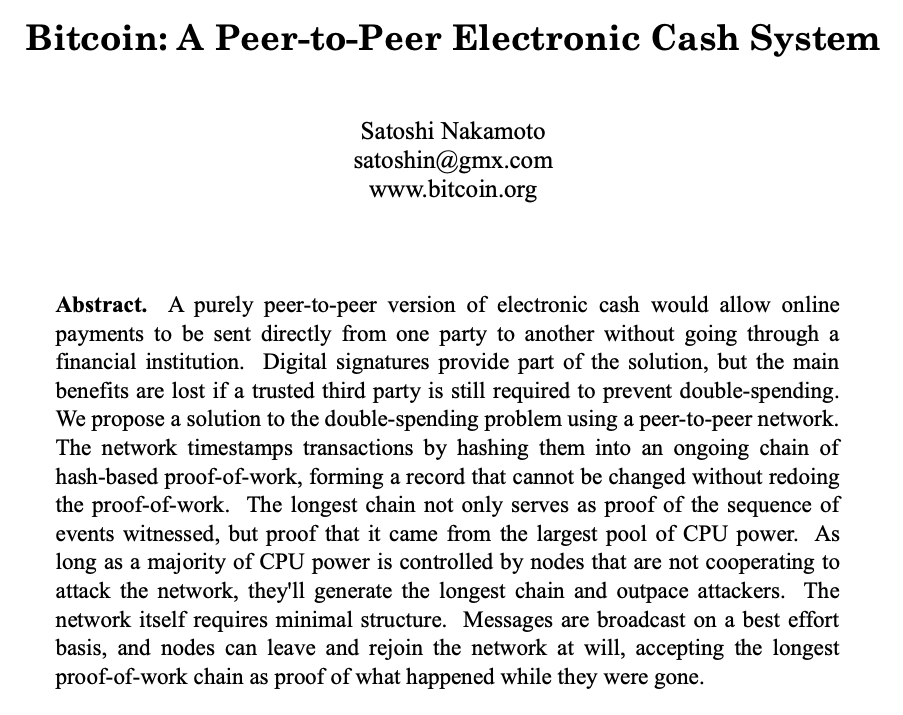
\includegraphics{img/btc-whitepaper.png}
  }
  \caption{Bitcoin Whitepaper by S. Nakamoto}
  \label{fig:btc-whitepaper}
\end{figure}
    \end{column}
  \end{columns}
\end{frame}

\begin{frame}{Définition générale}
  Blockchain se traduit par \textquote{chaîne de blocs}.
  Il s'agit donc d'un système permettant de stocker et de partager de l'information au travers d'un \textbf{structure de données bien choisie construite à partir de plusieurs blocs} (et c'est tout).

  La majorité des systèmes de blockchain possèdent des caractéristiques supplémentaires qui sont utilisées par abus de langage :

  \begin{enumerate}
    \item Présence d'une cryptomonnaie liée à la blockchain (il existe des blockchains SANS cryptomonnaies)
    \item Décentralisation
    \item Autonome/sans administration centrale
    \item Anonymat/pseudonimat des utilisateurs
  \end{enumerate}
\end{frame}

\begin{frame}{Définitions tierces}
  economie.gouv.fr
  \begin{quote}
    Développée à partir de 2008, c'est, en premier lieu, une technologie de stockage et de transmission d’informations. Cette technologie offre de hauts standards de transparence et de sécurité car elle fonctionne sans organe central de contrôle.

    Plus concrètement, la chaîne de blocs permet à ses utilisateurs - connectés en réseau - de partager des données sans intermédiaire.
  \end{quote}


  Wikipédia
  \begin{quote}
    Une blockchain, ou chaîne de blocs, est une technologie de stockage et de transmission d'informations sans autorité centrale. Techniquement, il s'agit d'une base de données distribuée dont les informations envoyées par les utilisateurs et les liens internes à la base sont vérifiés et groupés à intervalles de temps réguliers en blocs, formant ainsi une chaîne.
  \end{quote}
\end{frame}

\begin{frame}{Centralisation}
  Exemples:

  \begin{enumerate}
    \item L'Euro: la banque centrale européenne est souveraine et peut émettre des euros
    \item La force nucléaire en France : contrôlée par l'armée
    \item Twitter : la direction peut décider de retirer des privilèges sans l'approbation des utilisateurs (arrivée d'Elon Musk...)
  \end{enumerate}

  \begin{itemize}
    \item[$\Rightarrow$] La centralisation place un privilège/pouvoir entre les mains d'un petit groupe
    \item[$\Rightarrow$] Inversement, les utilisateurs sont tributaire du bon vouloir/bon fonctionement des systèmes
    \item[$\Rightarrow$] Une relation de \textbf{confiance} est nécessaire
  \end{itemize}
\end{frame}